\documentclass[conference]{IEEEtran}
\IEEEoverridecommandlockouts
% The preceding line is only needed to identify funding in the first footnote. If that is unneeded, please comment it out.
\usepackage{cite}
\usepackage{amsmath,amssymb,amsfonts}
\usepackage{algorithmic}
\usepackage{graphicx}
\usepackage{textcomp}
\usepackage{xcolor}
\usepackage{verbatim}
\usepackage{hyperref}
\def\BibTeX{{\rm B\kern-.05em{\sc i\kern-.025em b}\kern-.08em
    T\kern-.1667em\lower.7ex\hbox{E}\kern-.125emX}}
\begin{document}

\title{Breaking the Linear Barrier: A Multi-Modal LLM-Based System for Navigating Complex Web Content}

% \author{\IEEEauthorblockN{Gabriel Moterani}
% \IEEEauthorblockA{\textit{Digital Healthcare Innovation Lab} \\
% \textit{Faculty of Computer Science and Technology} \\
% \textit{Algoma University}\\
% Brampton, Canada \\
% gamorimmoterani@algomau.ca}
% \and
% \IEEEauthorblockN{Wenjun (Randy) Lin}
% \IEEEauthorblockA{\textit{Digital Healthcare Innovation Lab} \\
% \textit{Faculty of Computer Science and Technology} \\
% \textit{Algoma University}\\
% Brampton, Canada \\
% randy.lin@algomau.ca}
% }

\maketitle

\begin{abstract}
Visually impaired users still face fundamental obstacles when interacting with complex, dynamic websites. Conventional screen readers expose pages in a strict linear order, offer little semantic context for visual media, and provide limited support for completing multi‑step tasks. This paper introduces a multimodal accessibility framework combining Large Language Models (LLMs), Computer Vision, and dynamic DOM manipulation to significantly enhance semantic clarity, non-linear navigation, and interaction richness. By interpreting visual and textual web content contextually and adapting it into an intuitive, conversationally navigable interface, our method provides a foundation for visually impaired users to interact effectively with previously inaccessible or challenging digital experiences.

A working prototype deployed on a highly interactive tourism website demonstrated marked gains in content comprehension, navigation efficiency, and user autonomy, allowing blind participants to locate key information and purchase tickets without external assistance. By illustrating how vision–language reasoning can be coupled with low‑level browser control, this work lays the groundwork for future efforts in performance optimization, large‑scale evaluation, and personalization across diverse web contexts.
\end{abstract}

\begin{IEEEkeywords}
Web Accessibility, LLM, Accessibility DOM, Human-Computer Interaction, Context-Aware Systems
\end{IEEEkeywords}

\section{Introduction}

Despite the long-standing availability of web accessibility guidelines and assistive technologies, visually impaired users continue to face substantial challenges in navigating and interacting with contemporary websites. These challenges persist even as awareness and technological capabilities have advanced. Notably, 88\% of websites on the World Wide Web are still not accessible, reflecting a persistent gap between inclusive design principles and their real-world application \cite{webaccess2024}.

A key reason for this disconnect lies in the limitations of traditional assistive tools such as screen readers. These systems rely on linear content interpretation, which struggles with the complexity and interactivity of modern web experiences—particularly on platforms that depend on multimedia content, multi-step forms, or dynamically updated dashboards. Compounding the issue is the inconsistent implementation of accessibility standards such as the Web Content Accessibility Guidelines (WCAG), most recently updated with WCAG 3.0 in 2024. While these guidelines offer a robust framework for accessible design, their application often falls short due to a lack of developer expertise, improper use of ARIA (Accessible Rich Internet Applications) tags, and a prevailing focus on visual aesthetics rather than semantic clarity \cite{gbd2021, wcagchallenges2025}.

Recent advancements in context-aware technologies—such as LLM, Computer Vision, and Machine Learning—introduce new possibilities for bridging this accessibility gap. These technologies can supplement traditional assistive tools by acting as intelligent agents capable of interpreting, restructuring, and interacting with web content in real-time. Such systems can dynamically adapt interfaces to align with users' goals, offering not only improved content understanding but also richer forms of interaction.

In this work, we present a browser-based accessibility system powered by a multimodal architecture that integrates vision-language reasoning, contextual manipulation, and dialog-based task planning. Our system, implemented as a Google Chrome extension, enhances both the structure and semantics of web content. This system operates collaboratively across the Document Object Model (DOM) and the browser's Accessibility Tree, providing visually impaired users with the ability to more efficiently browse, comprehend, and interact with web content.

The remainder of this paper is organized as follows: Section II \ref{review} reviews related work and accessibility technologies; Section III details the proposed system and its modular architecture; Section IV describes the implementation methodology; Section V presents a practical usage scenario demonstrating the system in action; and Section VI concludes with findings, limitations, and directions for future research.


\section{Literature Review}\label{review}

Multiple studies over the past two decades have documented how screen readers process web pages strictly in a linear sequence, forcing visually‑impaired users to traverse headings, menus, and decorative elements before reaching relevant content. Large‑scale audits continue to report widespread keyboard‑navigation barriers, even on sites that advertise compliance with success criteria in WCAG 2.x and the 2024 WCAG 3.0 draft \cite{kerdar2024,wcagchallenges2025}. Empirical user observations show that the absence of semantic grouping leads to excessive keystrokes and cognitive overload when interacting with dashboards, multi‑column news layouts, and e‑commerce grids. Despite incremental improvements in screen‑reader software, the underlying linear traversal model remains unchanged—leaving the fundamental navigational burden on the user.

Accessible design guidelines require developers to supply meaningful alternative text, ARIA roles, and programmatic relationships, yet field surveys reveal that these elements are either missing or optimised for search‑engine ranking rather than human comprehension \cite{wcag2023}. Where alt text is present, it is often terse ("image1") or redundant with surrounding captions, providing little help in grasping complex visuals such as charts, infographics, or hero banners. Even on sites that partially implement WCAG techniques, dynamic content injected by third‑party ad networks or CMS templates escapes validation, breaking reading order and semantic context \cite{wcagchallenges2025}. As a result, visually‑impaired users must infer meaning from fragments that were never authored with their experience in mind.

Recent prototypes illustrate how LLM, computer vision, and DOM automation can enrich accessibility beyond traditional screen readers. Commercial and research extensions now parse shopping pages to surface product attributes in a simplified view, reducing navigation steps \cite{prakash2024}. Task‑oriented agents powered by LLMs translate natural‑language commands into browser actions, demonstrating promise in filling out forms, filtering tables, or performing multi‑step tasks \cite{kodandaram2024,mehendale2024}. While these systems validate the feasibility of AI‑mediated assistance, they remain domain‑specific, rely on brittle heuristics, or lack an integrated mechanism for maintaining conversational context across page transitions.

\subsection*{Synthesis and Identified Gaps}

Taken together, the literature confirms that technical progress has not yet resolved several critical barriers:

\begin{enumerate}
\item \textbf{Non‑linear navigation is still unsupported.} Screen readers continue to expose content in a purely sequential manner, forcing users through irrelevant elements before they reach task‑relevant information \cite{kerdar2024,wcagchallenges2025}.  
\item \textbf{Semantic context for visual content is insufficient.} Alt text and ARIA labels are inconsistently authored, providing at best superficial descriptions that fail to convey rich visual meaning \cite{wcag2023,wcagchallenges2025}.  
\item \textbf{General‑purpose, task‑driven interaction remains elusive.} AI‑augmented tools demonstrate success in narrow domains but do not yet offer a unified solution for complex, cross‑site workflows \cite{prakash2024,kodandaram2024,mehendale2024}.  
\end{enumerate}

Addressing these gaps motivates the multimodal, dialog‑centric system presented in this paper, which combines vision‑language reasoning, contextual DOM restructuring, and automated interaction execution to deliver an accessible yet fully interactive web experience for visually‑impaired users.



\section{Proposed System Overview}

While browsing the internet, users rely on software applications capable of facilitating data exchange with cloud servers via the Hypertext Transfer Protocol (HTTP), ultimately acquiring Hypertext content formatted in Hypertext Markup Language (HTML). These applications convert the textual representation of web pages into a visual format. These software applications are denominated as web browsers. At present, Google Chrome constitutes the primary browser utilized within desktop environments, accounting for a 66\% \cite{browserstats2025} market share. Conversely, Safari is predominantly used on mobile platforms employed by 22\% \cite{browserstats2025} of mobile users.

Web browsers have evolved to facilitate applications that function in conjunction with the product through the utilization of browser APIs. These applications, known as extensions, are installable within browsers and serve to augment the overall capabilities of the browser. Extensions enable developers to create enhancements for standard navigation, facilitating features such as text grammar correction, ad blockers, and other mechanisms. In this project, extensions are employed to interact with the DOM, which is the technical representation of elements on a web page in browsers, as well as the Accessibility Tree, which shares the same representation but is focused on what text-to-speech (TTS) mechanisms utilize to convert content for visually impaired users.

As shown in \autoref{tab:architecture}, our architecture orchestrates four cooperative modules around a shared task graph and state log. The LLM serves as the reasoning core, translating between raw pixels/DOM, natural‑language dialog, and low‑level interaction events.

\subsection{Visual‑Layout Interpreter (VLI)}
The VLI ingests periodic screenshots plus DOM snapshots, produces a hierarchical scene graph (regions, widgets, affordances), and assigns semantic tags using vision‑language prompting.

\subsection{Contextual Modification Engine (CME)}

The CME interrogates the scene graph, selects nodes pertinent to the task in progress, and adjusts the DOM elements with the objective of producing a more refined version of the Accessibility Tree that incorporates contextual descriptions alongside the application of WCAG compliance features, such as ARIA tags, CSS adjustments, and tag modifications.

\subsection{Conversational Plan Manager (CPM)}

The CPM runs a mixed‑initiative chat: it elicits the user's intent, decomposes it into subtasks using LLM reasoning, and writes an executable plan with checkpoint markers into the log.

\subsection{Multimodal Interaction Executor (MIE)}

The MIE iterates through the plan, emitting OS‑level events (e.g., pyautogui calls). After every action it requests an updated scene graph from the VLI to confirm success; discrepancies trigger CPM‑led replanning.


\begin{table}[ht]
\centering
\caption{System Components and Their Roles}
\label{tab:architecture}
\small
\renewcommand{\arraystretch}{1.5}
\begin{tabular}{|c|p{1.6cm}|p{1.6cm}|p{4cm}|}
\hline
\textbf{\#} & \textbf{Functional Role} & \textbf{Suggested Name} & \textbf{Rationale (concise)} \\
\hline
1 & Visual understanding of the current page & Visual‑Layout Interpreter (VLI) & Parses the rendered page bitmap/DOM into a structured semantic graph usable by language and planning components. \\
\hline
2 & Task‑aware presentation of information & Contextual Modification Engine (CME) & Re‑orders and summarizes page content according to the user's current goal (e.g., "browse headlines", "locate checkout button"). \\
\hline
3 & Dialogic intent capture \& planning & Conversational Plan Manager (CPM) & Conducts a mixed‑initiative dialog to clarify the user's objective, decomposes it into an executable plan, and maintains a progress log. \\
\hline
4 & Autonomous action execution & Multimodal Interaction Executor (MIE) & Carries out the CPM's plan (clicks, typing, drag‑and‑drop, drawing), and after each step re‑invokes the VLI to verify success or recover. \\
\hline
\end{tabular}
\vspace{0.5cm}
\end{table}


\subsection*{Example Workflow}

During the system's development, multiple visually impaired individuals were consulted regarding challenging tasks encountered on the internet. A prevalent issue identified was the navigation of online news sites. Despite developers' attempts to enhance accessibility, the dynamic elements, such as advertisements and diverse news services, render navigation overwhelming and nearly unmanageable. The transient nature of news, coupled with the vast volume of content produced, significantly impedes content adaptation for visually impaired users. 

In this scenario, we are modeling the basic process of accessing a news website to obtain insights regarding the essential conclusions of the most significant articles, as demonstrated in \autoref{tab:sequence}.

\vfill
\begin{table}[ht]
\centering
\caption{Phase and Module Sequence}
\label{tab:sequence}
\footnotesize
\renewcommand{\arraystretch}{2}
\begin{tabular}{|c|p{5.5cm}|}
\hline
\textbf{Phase} & \textbf{Module Sequence} \\
\hline
Intent capture & CPM → user: "What would you like to do?" → user: "Read today's headlines." \\
\hline
Context analysis & VLI parses home page; CME adapts headline list. \\
\hline
Choice \& plan & user: "Open the article about the lunar eclipse." → CPM drafts plan, seeks confirmation. \\
\hline
Execution \& feedback & MIE clicks headline; VLI validates article view; CME summarizes article; loop continues. \\
\hline
\end{tabular}
\vspace{0.5cm}
\end{table}

\section{Methodology}

An advanced architectural technology has been formulated to engineer a concise yet efficacious instrument aimed at augmenting navigational capabilities for individuals with visual impairments. This architecture can be methodically categorized into two primary structures: Front-end Development and Back-end Development.

The Front-end architecture facilitates the interaction between the browser and the tool, involving the extraction of data from the page, its transformation into pertinent nodes, and the establishment of interactions between the system-page and the user-system.

\subsection{Front-end Structure}

In the process of constructing the Front-end architecture, a comprehensive investigation into frameworks was undertaken to identify those that would offer enhanced performance and maintainability for the tool, as well as competence in interfacing with browser APIs effectively. The Plasmo framework for web extension development was selected as the foundational technology for the extension's creation. Plasmo integrates the web-ext library to facilitate the development of extensions using Javascript and Typescript languages, enabling the incorporation of sophisticated frontend libraries such as Reactjs. The amalgamation of these technologies empowered the developers to craft efficient, streamlined, and consistent interactions among pages, systems, and users.

Upon the rendering of a new page, the Front-end system detects alterations in the primary DOM elements, recognizing a modification and thereby activating the designated system to acquire both the DOM and Accessibility trees. This process involves filtering out superfluous content utilizing ad blocking technology and a readability library, a JavaScript library specifically designed to enhance readability by removing unnecessary content.

Since the technologies underpinning LLM depend on the volume of input text, which is converted into tokens — the fundamental units of LLM data — it is crucial that the frontend system sanitizes the input to supply the data interpreter with only essential information. Failure to do so necessitates that the content be divided into smaller segments for processing. This segmentation can result in increased rendering time of contextual elements, elevated server costs, and potential loss of context.

Subsequent to the purification of elements, the front-end will establish communication with the back-end modules through fundamental HTTPS requests. These modules will furnish the requisite context and information to be elaborated upon in the back-end subsection of this section. The front-end will then transform this contextual information into DOM modifications aimed directly at engaging with the Accessibility Tree, thereby enhancing the end-user experience. Furthermore, the extension will inject HTML elements into any web page, facilitating user interaction with the extension system, thereby enabling effective user-system communication and task execution by the system on behalf of the user.

\subsection{Back-end Structure}

The backend system is comprised of a Flask Python server configured to receive messages on port 8080. These messages are processed and converted into executable tasks for the system, resulting in outputs that are subsequently utilized by the Front-end in response to the queried messages. 

Although the backend encompasses a variety of techniques, it is essential to articulate four principal modules to provide clarity regarding its functionality.

\subsubsection{Visual Computation Methodology}

The server is tasked with receiving all visual elements, which may include binaries, image URLs, SVG (Scalable Vector Graphics) vectors, CSS (Cascading Style Sheets) cascade elements, or any other elements that pertain exclusively to a visual context. Based on the specific format of each element, the system processes these into images that are forwarded to a Computer Vision Machine Learning System. This system employs an algorithm that has been trained with an extensive dataset comprising billions of images, enabling it to accurately identify and describe the content within the images. The resulting image description is synthesized with a summary generated by an AI (Artificial Intelligence) language model, along with the proximate elements, to deliver a comprehensive contextual description of the visual element.

\subsubsection{Context Aware Methodology}

The server is responsible for receiving text, processed and queried by the Front-end from the DOM. This text is transmitted in JSON (JavaScript Object Notation) format and encompasses both the page content and the type of HTML tag encapsulating the text. The server then processes this information using a Large Language Model system, which extracts both the summary and additional context from the page. This refined information is subsequently utilized across various Back-end and Front-end modules throughout the system's operational workflow.

\subsubsection{WCAG Compliance Methodology}

The server's role involves receiving a JSON representation of DOM elements, upon which it processes this data through a finely tuned Large Language Model system. This LLM has been trained using data from websites exemplary of both effective and ineffective adherence to WCAG guidelines. Consequently, the LLM returns a JSON containing element identifiers and suggestions for compliance modifications or new tags. These alterations facilitate the conversion of the website's accessibility framework into a format that can be accurately interpreted by TTS systems. The front-end is then responsible for elucidating this information and accordingly transforming the page.

\subsubsection{RAG Conversational Task Executer Methodology}

Following the primary execution phase for context preparation, the server promptly stores a vector representation of the visited website. This vectorized model facilitates rapid and efficient communication with the AI, which is powered by a large language model (LLM). The content is queried via the vector database using Retrieval-Augmented Generation (RAG), enabling the identification of specific portions of the HTML code necessary for various tasks solicited by users. It subsequently returns executable actions via JavaScript. The frontend, equipped with this information, utilizes JavaScript commands to perform tasks on behalf of visually impaired users.


\begin{figure}[h]
\centerline{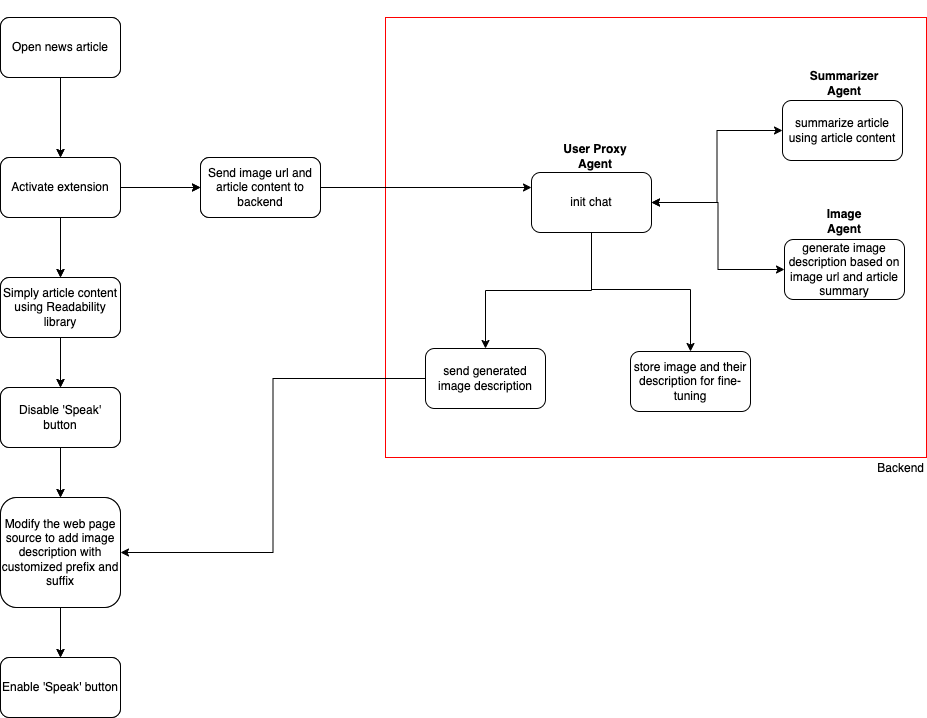
\includegraphics[width=\linewidth]{images/img1.png}}
\caption{Simplification of the Backend - Frontend Communication.}
\label{fig1}
\end{figure}

\section{Prototype Demonstration}

The presented example workflow aims to elucidate a straightforward task that can be performed by any user seeking to obtain fundamental information regarding the acquisition of data. In this prototype demonstration, we will simulate the challenges encountered by a visually impaired individual in comprehending the complete contextual information of the skywalk attraction at the CN Tower, a prominent landmark in Toronto. Following the installation of the Google Chrome extension, the DOM elements will undergo modification, resulting in alterations to the accessibility tree.

 Using this example we can prototype and display the proposed changes in the DOM. After using a basic google search about CN Tower Skywalk we encounter in the first result the following link:
 https://www.cntower.ca/brave-the-edgewalk

 \begin{figure}[h]
\centerline{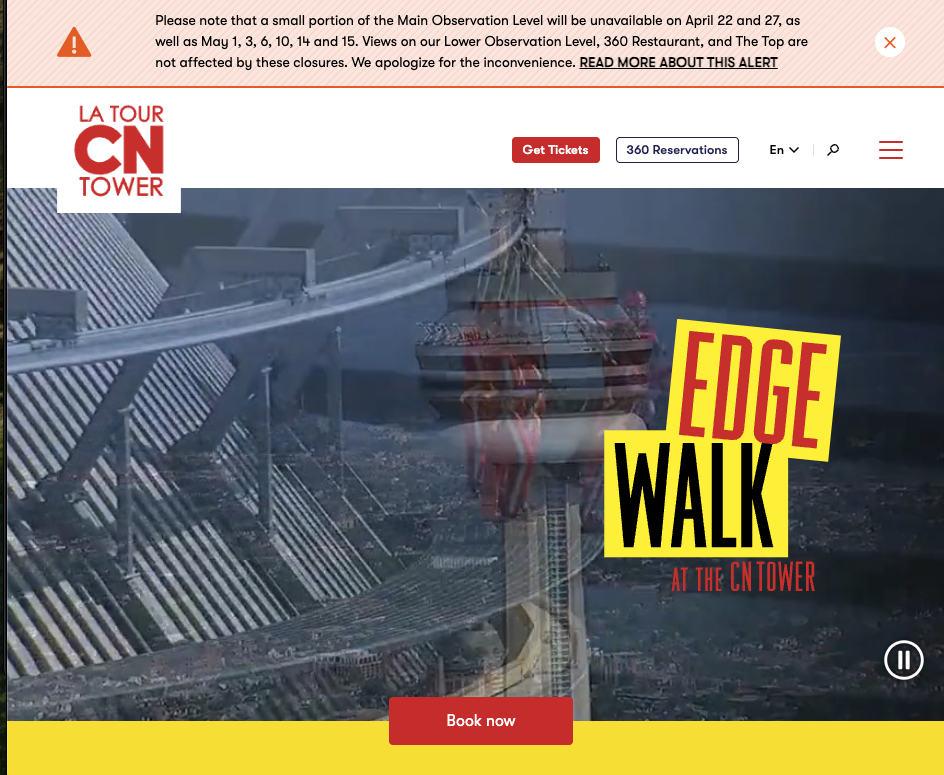
\includegraphics[width=\linewidth]{images/1.png}}
\caption{Skywak Landing Page Printscreen}
\label{fig2}
\end{figure}

The website incorporates certain guidelines from the WCAG; however, it presents a challenge from the outset due to its intricate navigation structure, utilization of video content, and inadequate support for keyboard navigation.

\begin{figure}[h]
\centerline{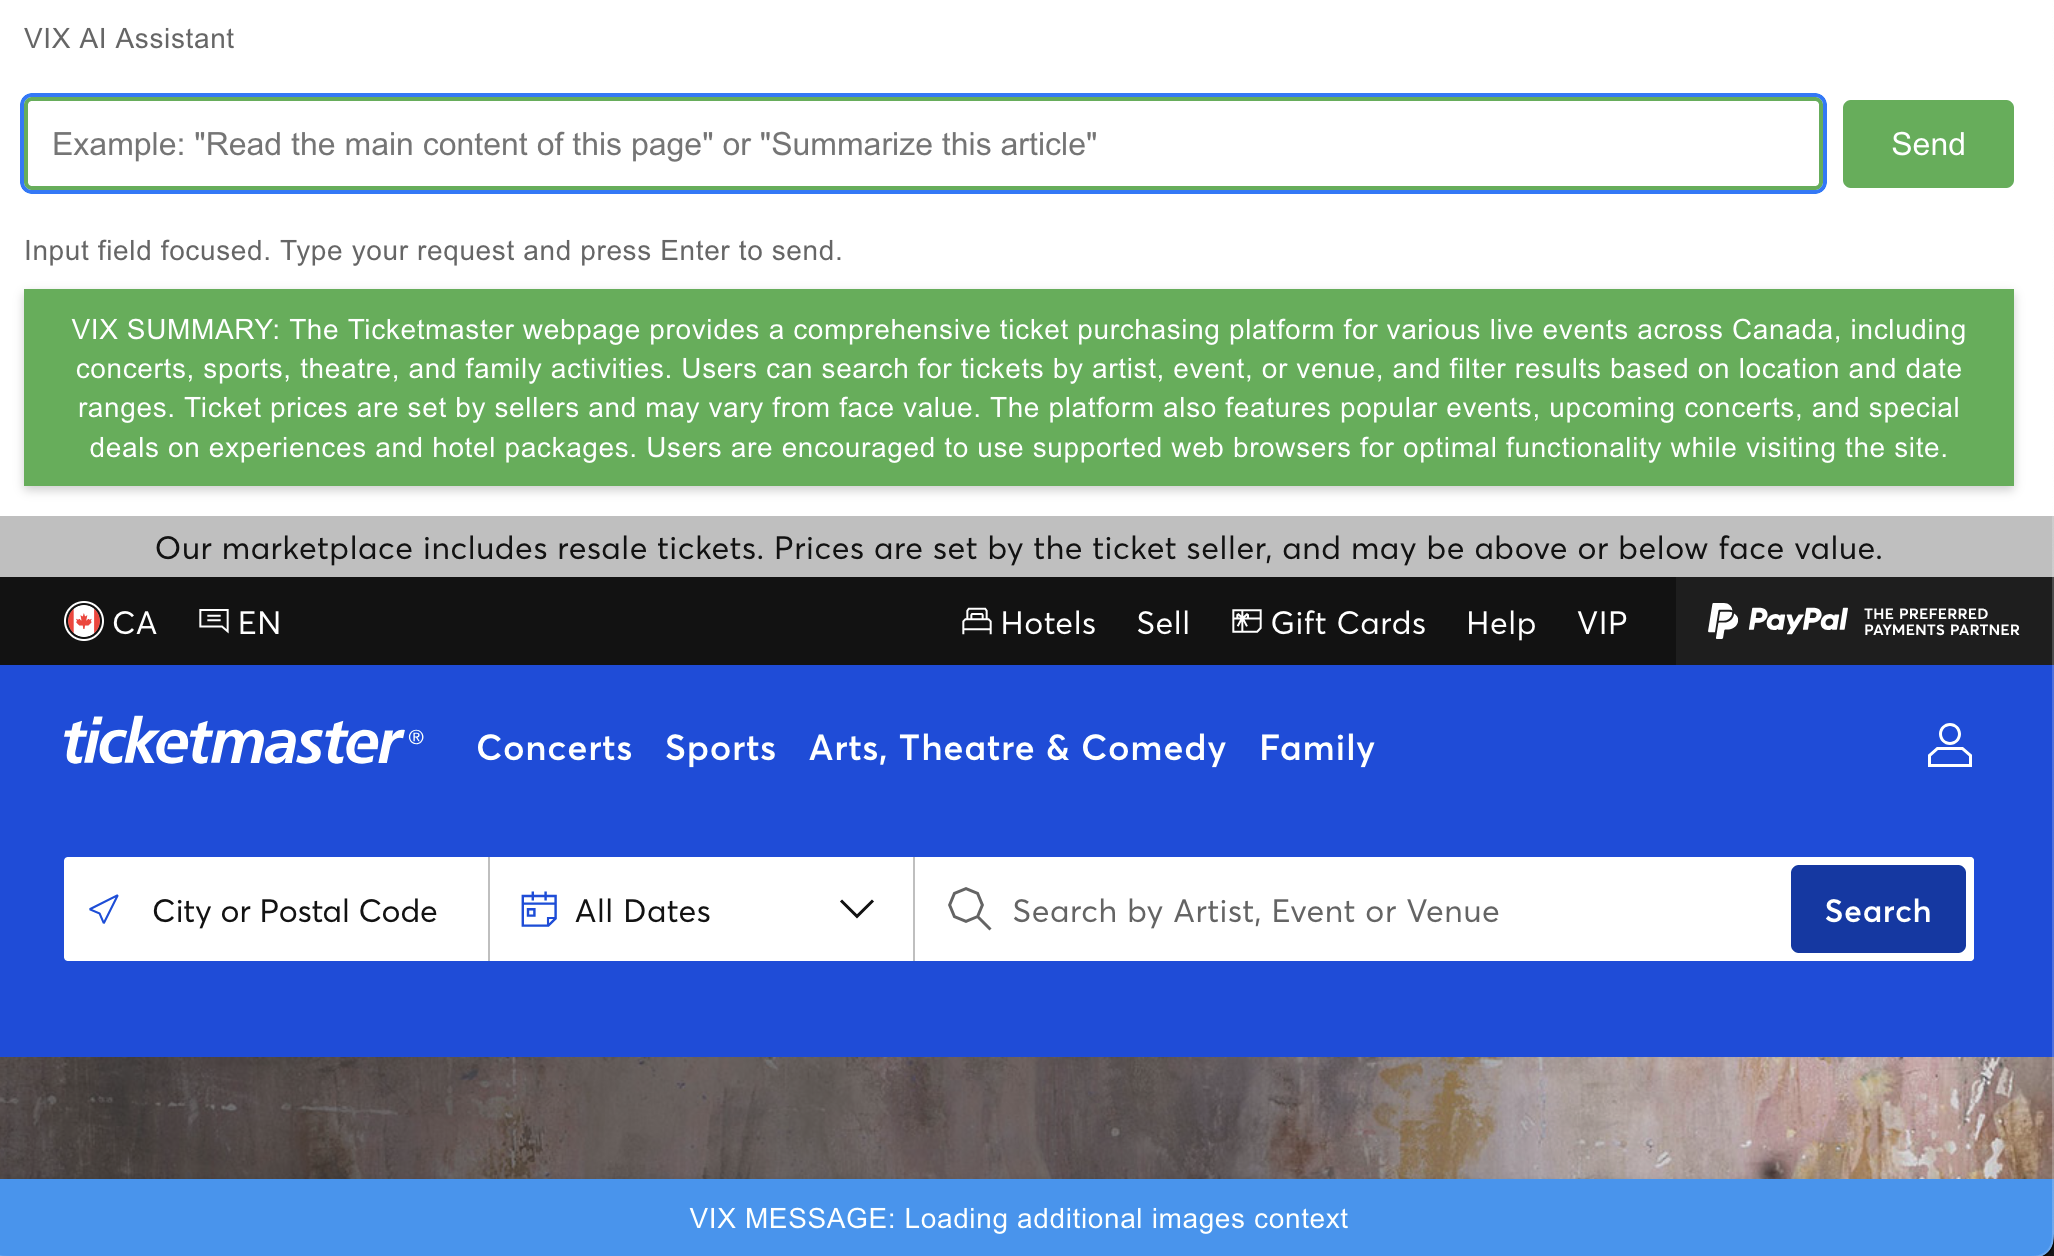
\includegraphics[width=\linewidth]{images/2.png}}
\caption{Page Use of Alternative Tags and Images}
\label{fig2}
\end{figure}

During navigation, users may encounter issues such as multiple layers of the same image being employed to facilitate expedited visual rendering for sighted users. However, in the accessibility DOM, these images are rendered multiple times. Furthermore, the alternative descriptions provided are brief and fail to deliver sufficient context regarding the intended event.

\begin{figure}[h]
\centerline{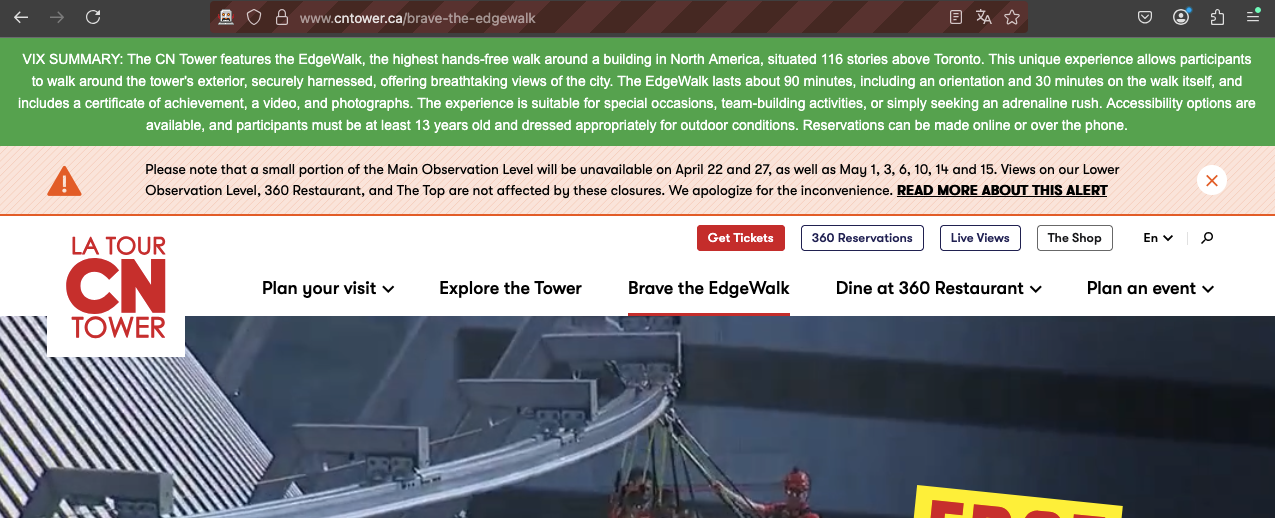
\includegraphics[width=\linewidth]{images/3.png}}
\caption{Summary Created by the Extension}
\label{fig2}
\end{figure}

After the page loading, extension starts rendering and parsing DOM elements, creating a new element with the summary of the page, that element is going to be rapidly parsed by the TTS assistive tools providing the user the ability to Scanning and Skimming content before trying to accomplish tasks in the page.

\begin{figure}[h]
\centerline{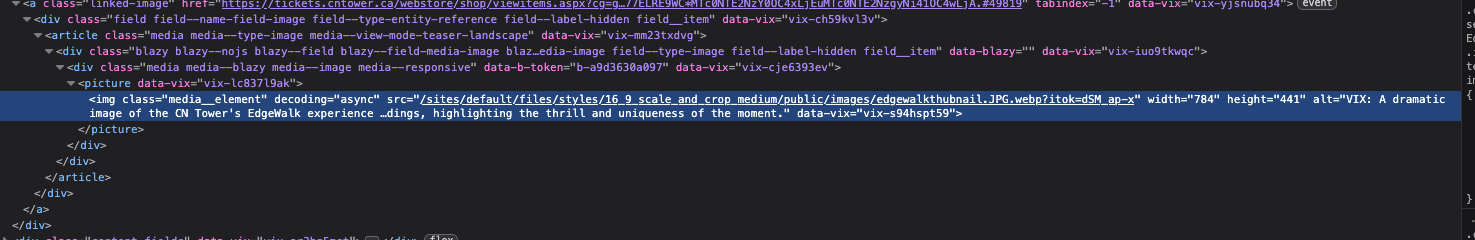
\includegraphics[width=\linewidth]{images/4.png}}
\caption{Parsed DOM Element}
\label{fig2}
\end{figure}

The extension subsequently analyzes images and visual elements, generating WCAG-compliant alternative tags and correcting ARIA tags to enhance navigability. It removes superfluous elements such as advertisements, visual embellishments, and other non-essential information from the DOM, thereby modifying the accessibility tree. Every tag will receive a new data-vix id in which the system will trust to query data to perform task.

Ultimately, users are now able to initiate a task via the extension, whereby the extension will parse the task and execute the necessary commands through JavaScript operations that engage with the webpage and the DOM.

\begin{figure}[h]
\centerline{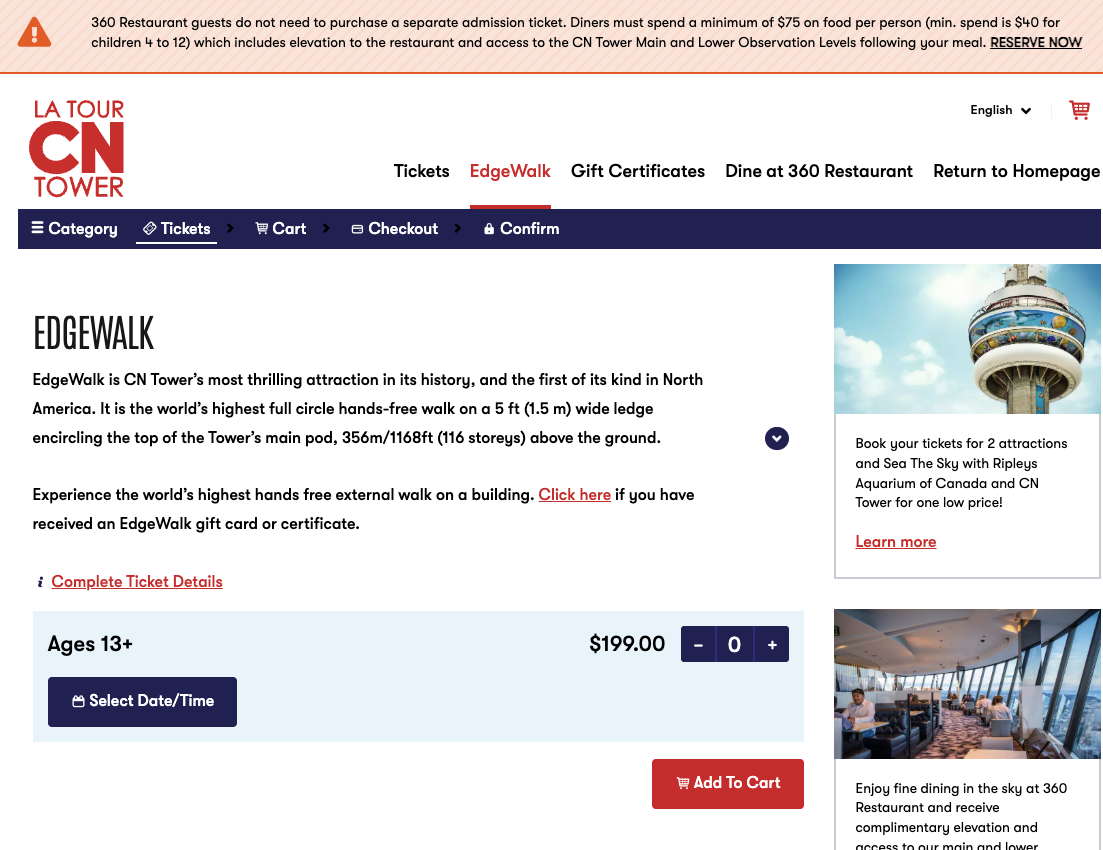
\includegraphics[width=\linewidth]{images/5.png}}
\caption{New Page with a new task of buying tickets}
\label{fig2}
\end{figure}

The user's task of acquiring information about the event is completed, and the user is redirected through the extension workforce to a new page, where the CN Tower is presented for the task of purchasing tickets. The system is available for repeated use to facilitate the acquisition of tickets.


\section{Conclusion}

This paper has addressed critical and persistent accessibility challenges experienced by visually impaired users navigating modern web environments. Through integrating advances in LLMs, computer vision, and dynamic DOM manipulation, we introduced a multimodal accessibility system designed as a browser extension to significantly enhance web interaction experiences for visually impaired users.

Our architecture uniquely combines four core modules—VLI, CME, CPM, and MIE—to collaboratively parse visual and semantic content, dynamically reorganize web page structures, conduct intent-based conversational planning, and automate complex web interactions. The prototype demonstration using the CN Tower Skywalk attraction webpage highlighted the system's practical capability to simplify complex navigation tasks, enhance semantic comprehension through improved alt text and ARIA labels, and successfully execute user-driven tasks such as information retrieval and ticket purchases.

However, despite its promising outcomes, several practical and technical limitations have been identified. First, the computational costs associated with real-time inference of LLM and computer vision models remain high, necessitating server resources equipped with high-performance GPUs (Graphics Processing Unit). Second, latency introduced by inter-module communication and iterative page rendering may affect usability during extensive interactions. Third, the prototype's ability to generalize its effectiveness across diverse web structures and complex dynamic websites requires further development and validation.

Future research directions are clear and critical for achieving broader adoption and usability. Optimizing system performance and reducing computational demands through more efficient inference methods and specialized LLM fine-tuning specifically for accessibility tasks are immediate priorities. Additionally, exploring expansions into mobile environments, multilingual contexts, and undertaking rigorous user studies involving visually impaired users will substantially enhance practical utility and real-world applicability.

Ultimately, while technical innovation forms the core of our approach, the broader vision remains creating a universally accessible internet. Emphasizing user-centered iterative development, ongoing collaboration, and inclusive design principles will ensure that advancements in AI technology translate meaningfully into equitable digital experiences for all users.


\section{Use of AI Disclosure}
No artificial intelligence tools were employed in the generation of the content presented in this document. Throughout the drafting process, the Overleaf IEEE AI Assistant was utilized to review grammatical accuracy and to offer feedback on writing style and consistency, thereby suggesting improvements to the text and making modifications to the content. During the coding phase of the project, Claude AI, version 3.5, was employed to assist developers in coding tasks and error resolution.


% References
\bibliographystyle{unsrt}
\bibliography{references}
\end{document}
